\newpage
\section{Front-End}
\label{QuizziPedia::Front-End}
\begin{figure}[ht]
	\centering
	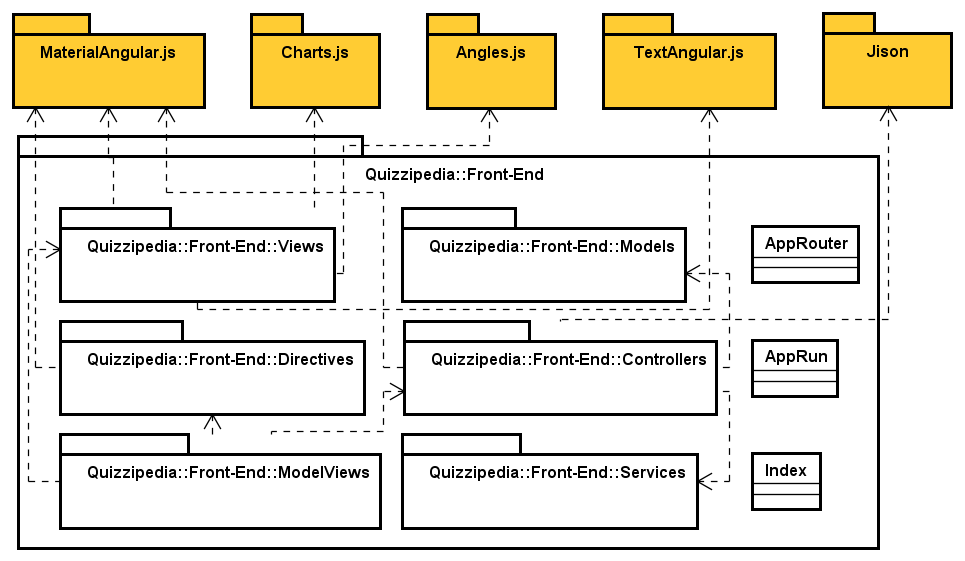
\includegraphics[scale=0.35]{UML/Package/QuizziPedia_Front-end.png}
	\caption{QuizziPedia::Front-End}
\end{figure}
\FloatBarrier
\begin{itemize}
	\item \textbf{Descrizione}: \textit{package\ped{G}} contenente le componenti front-end dell'applicazione;
	\item \textbf{Package contenuti}:
	\begin{itemize}
		\item \texttt{Controllers}: \textit{package\ped{G}} contenente i \textit{controllers\ped{G}} front-end dell'applicazione;
		\item \texttt{Directives}: \textit{package\ped{G}} contenente le \textit{directives\ped{G}} front-end dell'applicazione;
		\item \texttt{Models}: \textit{package\ped{G}} contenente le classi che definiscono la business logic dell'applicazione;
		\item \texttt{Services}: \textit{package\ped{G}} contenente i \textit{services\ped{G}} front-end dell'applicazione;
		\item \texttt{Views}: \textit{package\ped{G}} contenente le \textit{views\ped{G}} front-end dell'applicazione;
	\end{itemize}
\end{itemize}


